\documentclass{report}

\usepackage{graphicx}

\graphicspath{./}

\begin{document}
    \title  { \textbf{SYSC 4602 Assignment 1} }
    \author {
        David (student number),
        Ghassan (student number),
        Zach (101069001)
    }

    \maketitle

    \chapter*{Part 1: Capturing a Trace}
    \begin{figure}[h]
        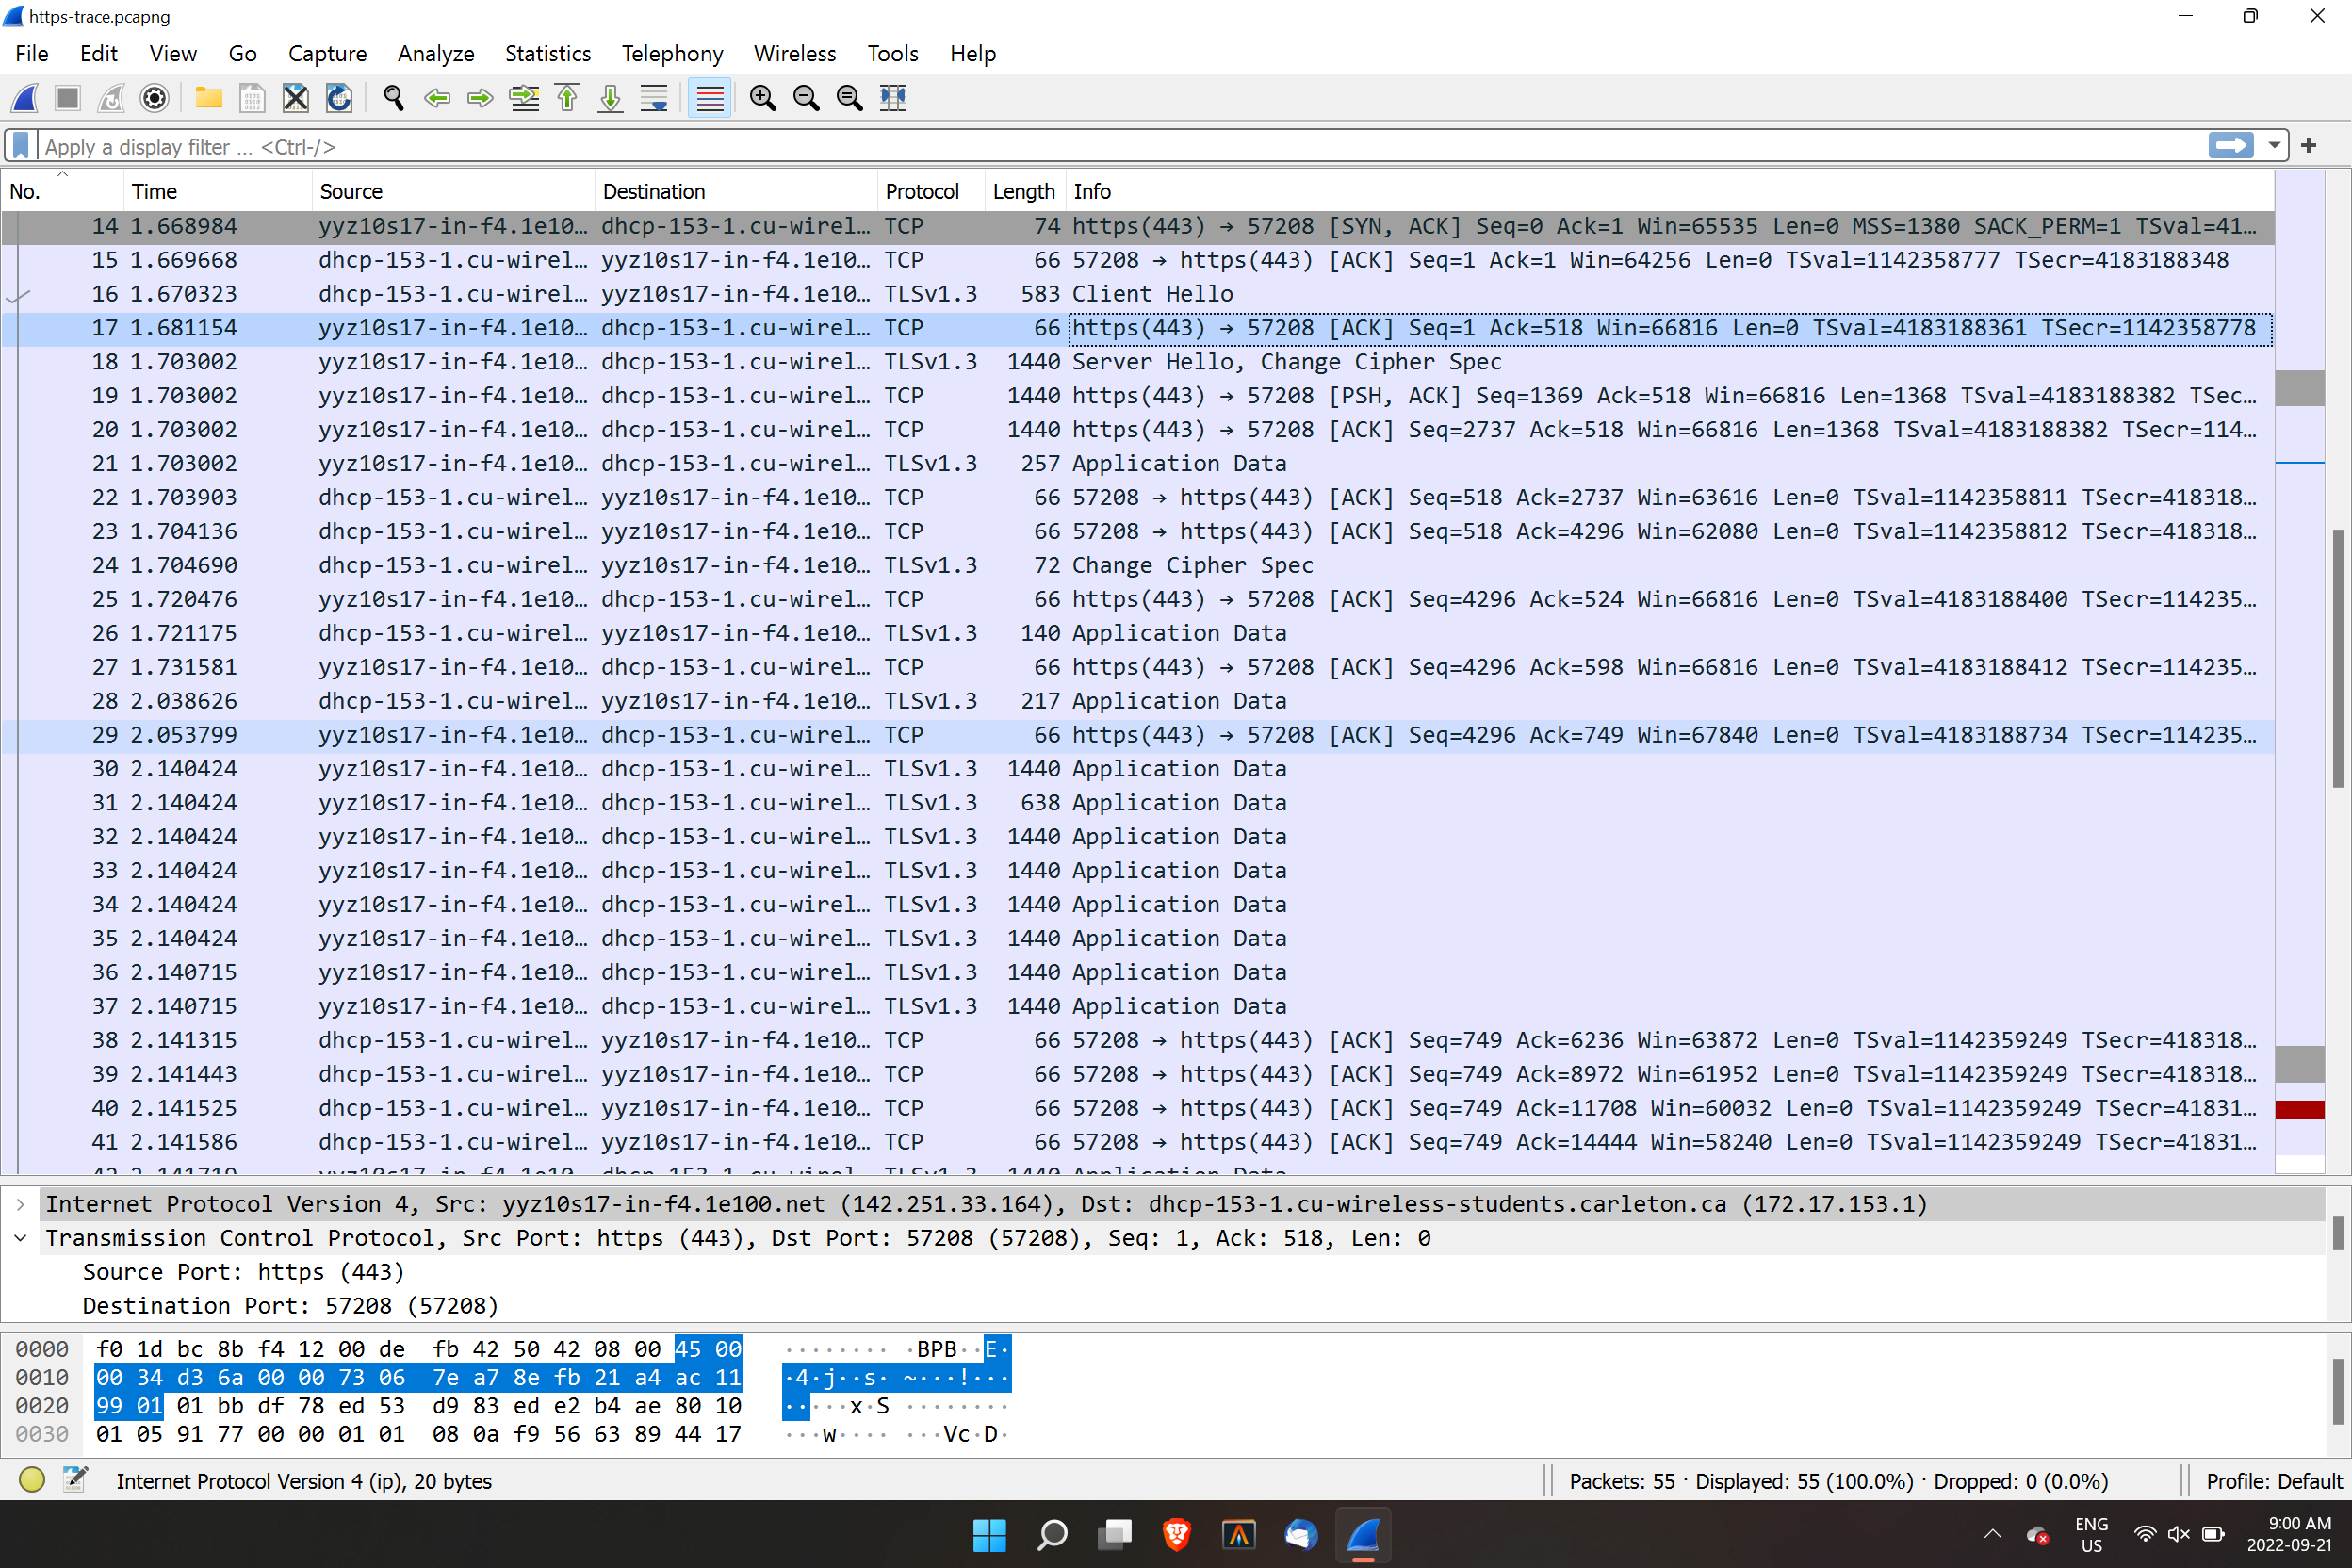
\includegraphics[width=\textwidth]{images/trace-https.png}
        \caption{Captured trace of wget https://www.google.com}
    \end{figure}

    \chapter*{Part 2: Inspecting the Trace}
    \begin{figure}[h]
        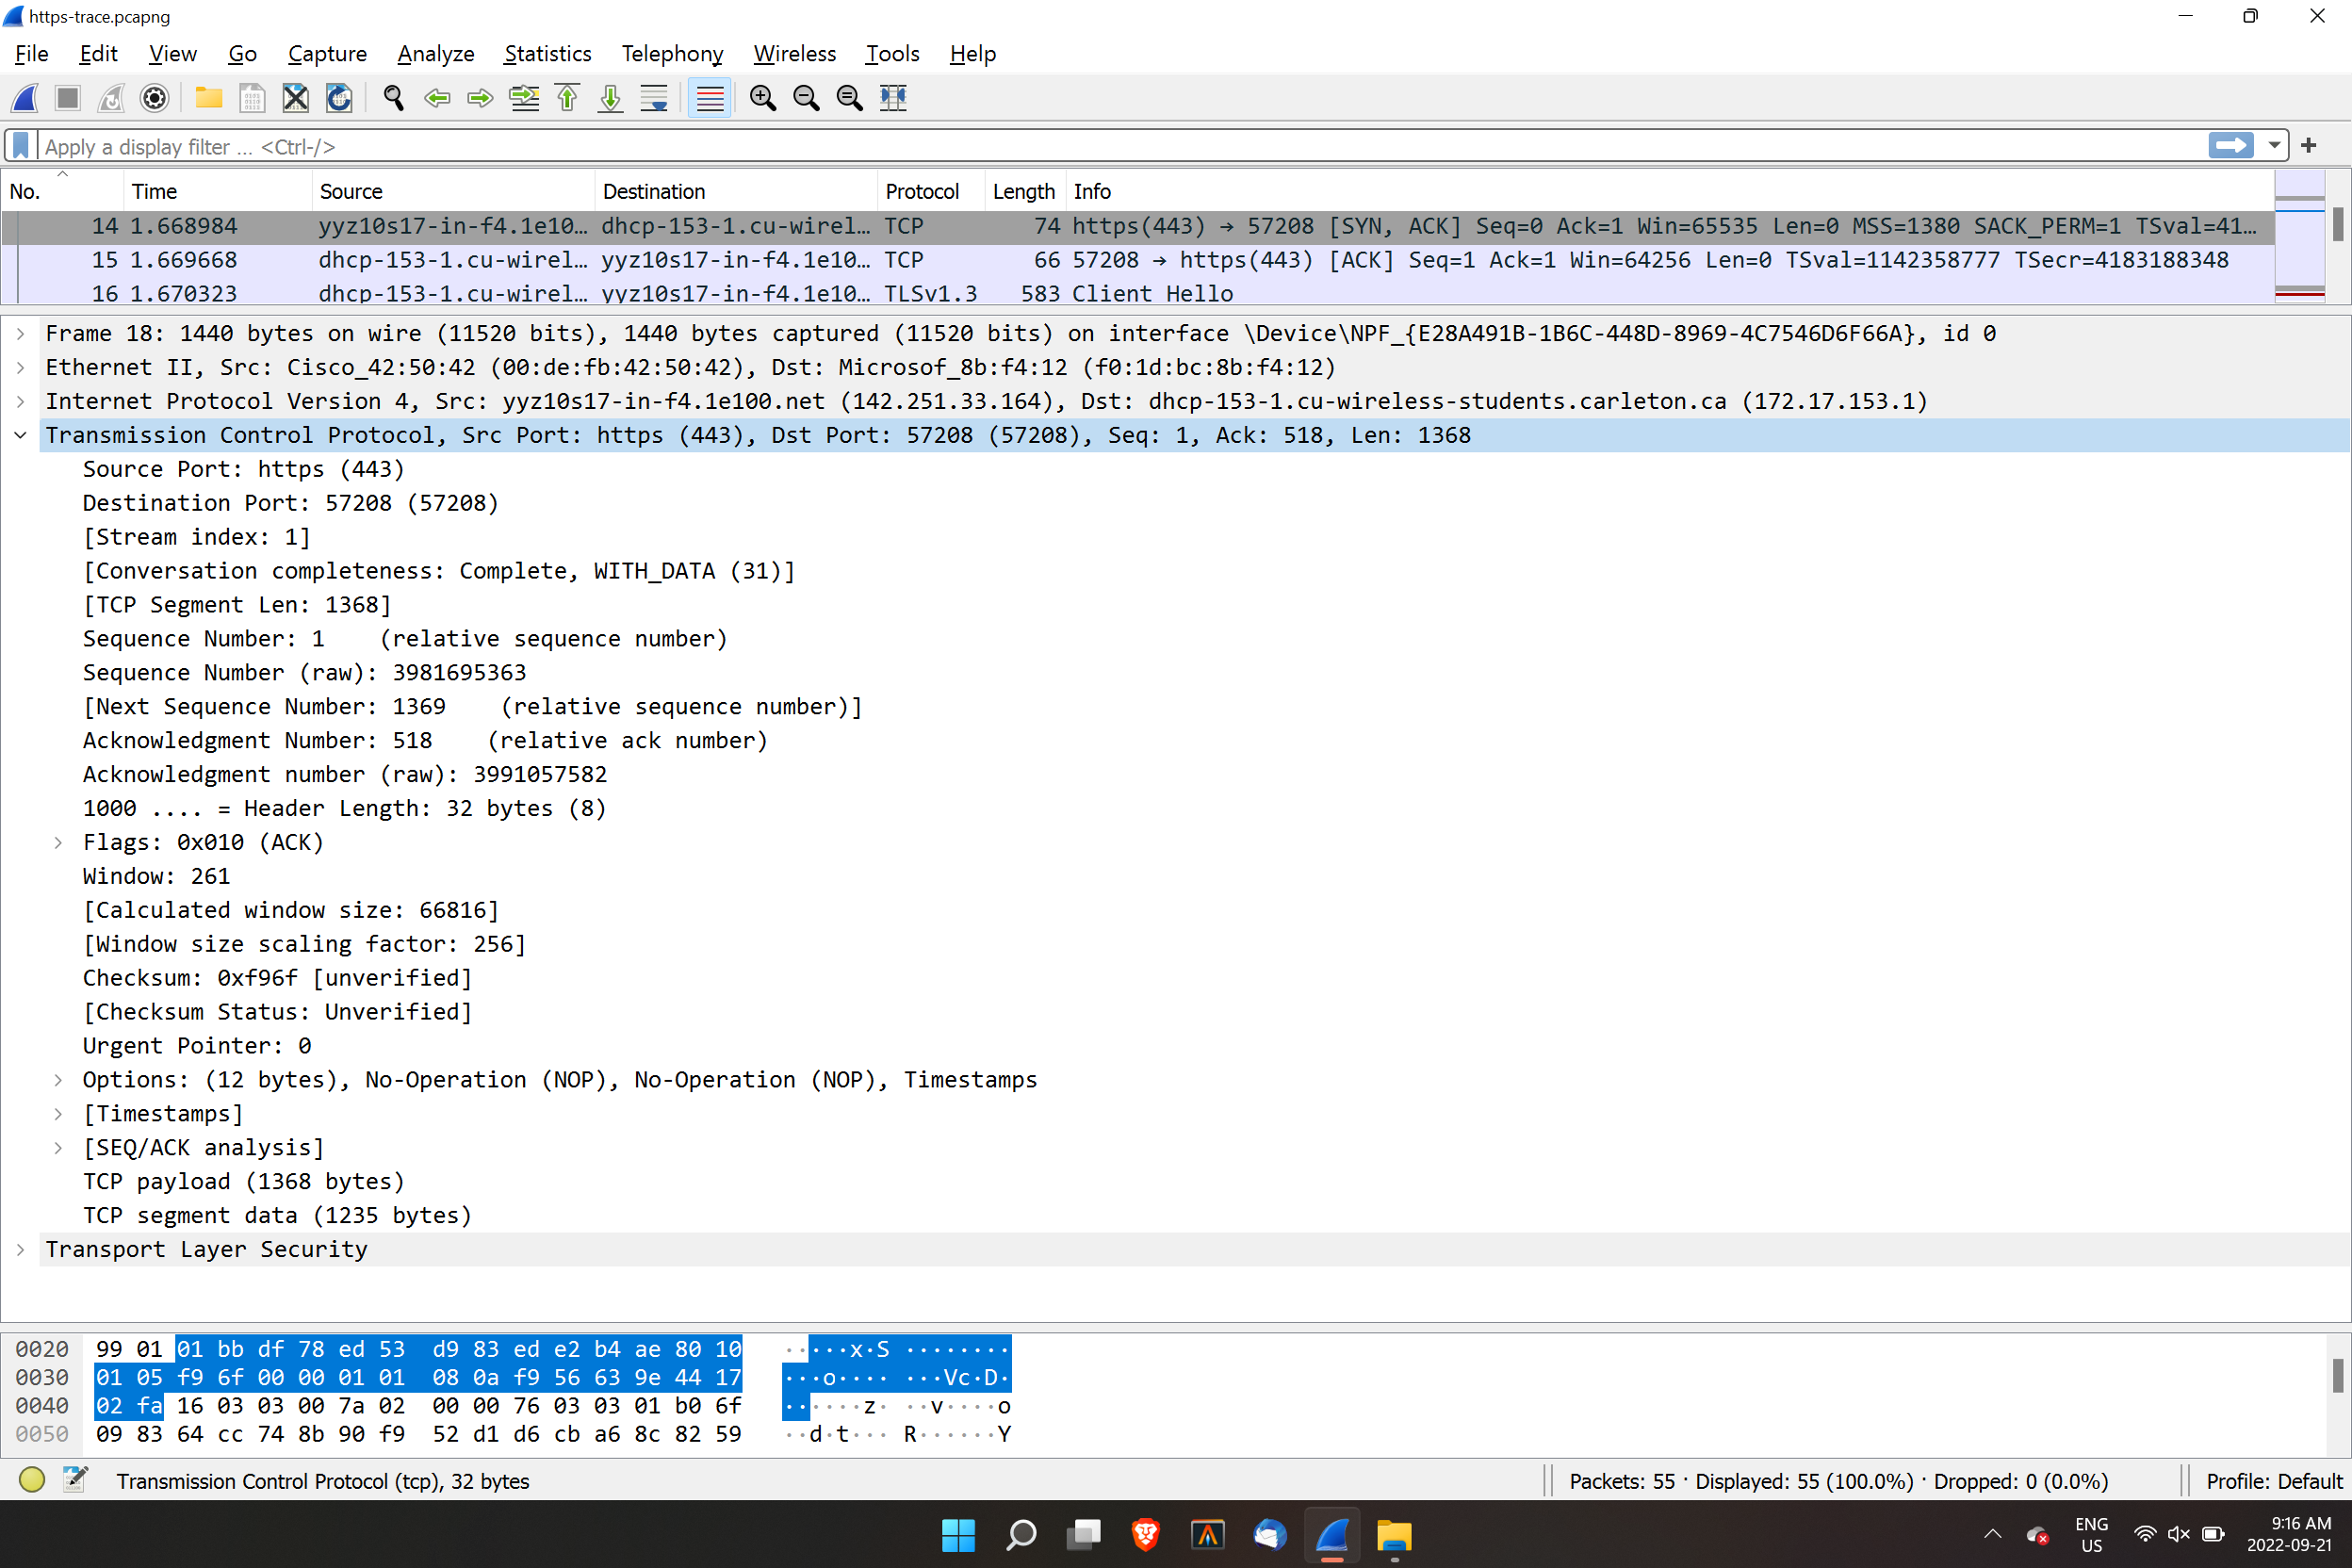
\includegraphics[width=\textwidth]{images/https-server-hello-structure-1.png}
        \caption{Packet structure of https Server Hello Packet}
    \end{figure}

    \chapter*{Part 3: Packet Structure}
    \begin{figure}[h]
        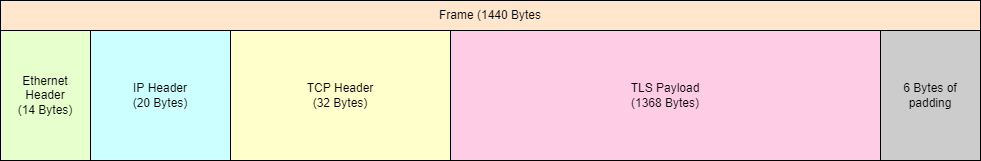
\includegraphics[width=\textwidth]{images/packet_structure.drawio.png}
        \caption{Packet Structure Diagram}
    \end{figure}
    \chapter*{Part 4: Protocol Overhead}

    total bytes = 23079\\
    total payload = 23014\\\\

    Ratio of payload to bytes = 23079 / 23014 = 99.7\%\\
    Amount of overhead = 100\% - 99.7\% = 0.3\%\\

    Therefore 0.3\% of the overall download is overhead.\\

    \chapter*{Part 5: Demultiplexing Keys}
    \section{}
    \subsection{}
    The Type field is the demultiplexing key for the ethernet header.\\

    The type field indicates IPv4 which corresponds to the IP header.\\

    \subsection{}
    The protocol field is the demultiplexing key for the IP header.\\

    The protocol field indicates TCP (6) which corresponds to the TCP header.\\

\end{document}
